% -----------------------------*- LaTeX -*------------------------------
\documentclass[UTF8]{report}
% ------------------------------------------------------------------------
% Packages
% ------------------------------------------------------------------------
\usepackage{adjustbox}
\usepackage{algorithm,algorithmicx}
\usepackage[noend]{algpseudocode}
\usepackage{amsmath,amsfonts,amssymb,bm,amsthm}%数学宏包、数学字体、数学符号、支持 \mathscr{} 字体、支持粗斜体 \bm{}、数学定理
\usepackage{bigstrut,multirow,rotating}%Excel表格自动导入latex
\usepackage{booktabs}
\usepackage{breqn}
\usepackage{caption}
\usepackage{color}%支持颜色改变
\usepackage{ctex}
\usepackage{enumitem}%自定义列表环境
\usepackage{esint}%支持多种积分算子
\usepackage{extarrows}%任意长度的箭头
\usepackage{fancyhdr}
\usepackage{fontsize}
\usepackage{fontspec}
\usepackage[body={7in, 9in},left=1in,right=1in]{geometry}
\usepackage{graphicx}%支持 \includegraphics{} 插图
\usepackage{mathrsfs}
\usepackage{mathtools}%数学宏包的重要补充
\usepackage[framemethod=TikZ]{mdframed}
\usepackage{nicefrac}
\usepackage{scribe}
\usepackage{subfigure}%插入子图
\usepackage{tikz,xcolor}%画图、画 Feynman 图
\usepackage{upgreek}%数学环境的直立希腊字母
% ------------------------------------------------------------------------
% Macros
% ------------------------------------------------------------------------
%~~~~~~~~~~~~~~~
% Utility latin
%~~~~~~~~~~~~~~~
\newcommand{\ie}{\textit{i.e.}}
\newcommand{\eg}{\textit{e.g.}}
%~~~~~~~~~~~~~~~
% Environment shortcuts
%~~~~~~~~~~~~~~~
\newcommand{\balign}[1]{\ealign{\begin{align}#1\end{align}}}
\newcommand{\baligns}[1]{\ealigns{\begin{align*}#1\end{align*}}}
\newcommand{\bitemize}[1]{\eitemize{\begin{itemize}#1\end{itemize}}}
\newcommand{\benumerate}[1]{\eenumerate{\begin{enumerate}#1\end{enumerate}}}
%~~~~~~~~~~~~~~~
% Text with quads around it
%~~~~~~~~~~~~~~~
\newcommand{\qtext}[1]{\quad\text{#1}\quad}
%~~~~~~~~~~~~~~~
% Shorthand for math formatting
%~~~~~~~~~~~~~~~
\newcommand{\mbb}[1]{\mathbb{#1}}
\newcommand{\mbi}[1]{\boldsymbol{#1}} % Bold and italic (math bold italic)
\newcommand{\mbf}[1]{\mathbf{#1}}
\newcommand{\mc}[1]{\mathcal{#1}}
\newcommand{\mrm}[1]{\mathrm{#1}}
\newcommand{\tbf}[1]{\textbf{#1}}
\newcommand{\tsc}[1]{\textsc{#1}}
%\def\<{{\langle}}
%\def\>{{\rangle}}
\newcommand{\sT}{\sf T}
\newcommand{\grad}{\nabla}
\newcommand{\Proj}{\Pi}
%~~~~~~~~~~~~~~~
% Common sets 定义数集符号
%~~~~~~~~~~~~~~~
\newcommand{\R}{\mathbb{R}}
\newcommand{\Z}{\mathbb{Z}}
\newcommand{\Q}{\mathbb{Q}}
\newcommand{\N}{\mathbb{N}}
\newcommand{\C}{\mathbb{C}}
\newcommand{\reals}{\mathbb{R}} % Real number symbol
\newcommand{\integers}{\mathbb{Z}} % Integer symbol
\newcommand{\rationals}{\mathbb{Q}} % Rational numbers
\newcommand{\naturals}{\mathbb{N}} % Natural numbers
\newcommand{\complex}{\mathbb{C}} % Complex numbers
%~~~~~~~~~~~~~~~
% Common functions
%~~~~~~~~~~~~~~~
\renewcommand{\exp}[1]{\operatorname{exp}\left(#1\right)} % Exponential
\newcommand{\indic}[1]{\mbb{I}\left(#1\right)} % Indicator function
\newcommand{\indicsub}[2]{\mbb{I}_{#2}\left(#1\right)} % Indicator function
\newcommand{\argmax}{\mathop\mathrm{arg\, max}} % Defining math symbols
\newcommand{\argmin}{\mathop\mathrm{arg\, min}}
\renewcommand{\arccos}{\mathop\mathrm{arccos}}
\newcommand{\dom}{\mathop\mathrm{dom}} % Domain
\newcommand{\range}{\mathop\mathrm{range}} % Range
\newcommand{\diag}{\mathop\mathrm{diag}}
\newcommand{\tr}{\mathop\mathrm{tr}}
\newcommand{\abs}{\mathop\mathrm{abs}}
\newcommand{\card}{\mathop\mathrm{card}}
\newcommand{\sign}{\mathop\mathrm{sign}}
\newcommand{\prox}{\mathrm{prox}} % prox
\newcommand{\rank}[1]{\mathrm{rank}(#1)}
\newcommand{\supp}[1]{\mathrm{supp}(#1)}
\newcommand{\norm}[1]{\lVert#1\rVert}
%~~~~~~~~~~~~~~~
% Common probability symbols
%~~~~~~~~~~~~~~~
\newcommand{\family}{\mathcal{P}} % probability family / statistical model
\newcommand{\iid}{\stackrel{\mathrm{iid}}{\sim}}
\newcommand{\ind}{\stackrel{\mathrm{ind}}{\sim}}
\newcommand{\E}{\mathbb{E}} % Expectation symbol
\newcommand{\Earg}[1]{\E\left[#1\right]}
\newcommand{\Esubarg}[2]{\E_{#1}\left[#2\right]}
\renewcommand{\P}{\mathbb{P}} % Probability symbol
\newcommand{\Parg}[1]{\P\left(#1\right)}
\newcommand{\Psubarg}[2]{\P_{#1}\left[#2\right]}
%\newcommand{\Cov}{\mrm{Cov}} % Covariance symbol
%\newcommand{\Covarg}[1]{\Cov\left[#1\right]}
%\newcommand{\Covsubarg}[2]{\Cov_{#1}\left[#2\right]}
%\newcommand{\model}{\mathcal{P}} % probability family / statistical model
%~~~~~~~~~~~~~~~
% Distributions
%~~~~~~~~~~~~~~~
%\newcommand{\Gsn}{\mathcal{N}}
%\newcommand{\Ber}{\textnormal{Ber}}
%\newcommand{\Bin}{\textnormal{Bin}}
%\newcommand{\Unif}{\textnormal{Unif}}
%\newcommand{\Mult}{\textnormal{Mult}}
%\newcommand{\NegMult}{\textnormal{NegMult}}
%\newcommand{\Dir}{\textnormal{Dir}}
%\newcommand{\Bet}{\textnormal{Beta}}
%\newcommand{\Gam}{\textnormal{Gamma}}
%\newcommand{\Poi}{\textnormal{Poi}}
%\newcommand{\HypGeo}{\textnormal{HypGeo}}
%\newcommand{\GEM}{\textnormal{GEM}}
%\newcommand{\BP}{\textnormal{BP}}
%\newcommand{\DP}{\textnormal{DP}}
%\newcommand{\BeP}{\textnormal{BeP}}
%\newcommand{\Exp}{\textnormal{Exp}}
%~~~~~~~~~~~~~~~
% Theorem-like environments
%~~~~~~~~~~~~~~~
%\theoremstyle{definition}
%\newtheorem{definition}{Definition}
%\newtheorem{example}{Example}
%\newtheorem{problem}{Problem}
%\newtheorem{lemma}{Lemma}
%~~~~~~~~~~~~~~~
% 组合数学的模板和作业里用到的一些宏包和自定义命令
%~~~~~~~~~~~~~~~
\renewcommand{\emph}[1]{\begin{kaishu}#1\end{kaishu}}
\newcommand{\falfac}[1]{^{\underline{#1}}}
\newcommand{\binomfrac}[2]{\frac{#1^{\underline{#2}}}{#2!}}
\newcommand{\ceil}[1]{\left\lceil #1 \right\rceil}
\newcommand{\floor}[1]{\left\lfloor #1 \right\rfloor}
\newcommand{\suminfty}[2]{\sum_{#1=#2}^{\infty}}
\newcommand{\suminftyk}[0]{\sum_{k=0}^{\infty}}
\newcommand{\sumint}[3]{\sum_{#1=#2}^{#3}}
\newcommand{\sumintk}[2]{\sum_{k=#1}^{#2}}
\newcommand{\suminti}[2]{\sum_{i=#1}^{#2}}
%~~~~~~~~~~~~~~~
% 定义新命令
%~~~~~~~~~~~~~~~
\newcommand*{\unit}[1]{\mathop{}\!\mathrm{#1}}
\newcommand*{\dif}{\mathop{}\!\mathrm{d}}%微分算子 d
\newcommand*{\pdif}{\mathop{}\!\partial}%偏微分算子
\newcommand*{\cdif}{\mathop{}\!\nabla}%协变导数、nabla 算子
\newcommand*{\laplace}{\mathop{}\!\Delta}%laplace 算子
\newcommand*{\deriv}[2]{\frac{\mathrm{d} #1}{\mathrm{d} {#2}}}
\newcommand*{\derivh}[3]{\frac{\mathrm{d}^{#1} #2}{\mathrm{d} {#3^{#1}}}}
\newcommand*{\pderiv}[2]{\frac{\partial #1}{\partial {#2}}}
\newcommand*{\pderivh}[3]{\frac{\partial^{#1} #2}{\partial {#3^{#1}}}}
\newcommand*{\dderiv}[2]{\dfrac{\mathrm{d} #1}{\mathrm{d} {#2}}}
\newcommand*{\dderivh}[3]{\dfrac{\mathrm{d}^{#1} #2}{\mathrm{d} {#3^{#1}}}}
\newcommand*{\dpderiv}[2]{\dfrac{\partial #1}{\partial {#2}}}
\newcommand*{\dpderivh}[3]{\dfrac{\partial^{#1} #2}{\partial {#3^{#1}}}}
\newcommand{\me}[1]{\mathrm{e}^{#1}}%e 指数
\newcommand{\mi}{\mathrm{i}}%虚数单位
%\newcommand{\mc}{\mathrm{c}}%光速 定义与mathcal冲突
\newcommand{\red}[1]{\textcolor{red}{#1}}
\newcommand{\blue}[1]{\textcolor{blue}{#1}}
%\newcommand{\Rome}[1]{\setcounter{rome}{#1}\Roman{rome}}
%~~~~~~~~~~~~~~~
% 公式环境中箭头符号的简写
%~~~~~~~~~~~~~~~
\newcommand{\ra}{\rightarrow}
\newcommand{\Ra}{\Rightarrow}
\newcommand{\la}{\leftarrow}
\newcommand{\La}{\Leftarrow}
\newcommand{\lra}{\leftrightarrow}
\newcommand{\Lra}{\Leftrightarrow}
\newcommand{\lgla}{\longleftarrow}
\newcommand{\Lgla}{\Longleftarrow}
\newcommand{\lgra}{\longrightarrow}
\newcommand{\Lgra}{\Longrightarrow}
\newcommand{\lglra}{\longleftrightarrow}
\newcommand{\Lglra}{\Longleftrightarrow}
%~~~~~~~~~~~~~~~
% 本.tex文档中特殊定义命令
%~~~~~~~~~~~~~~~
\newcommand{\cdclass}[2]{[#1]_{\text{#2}}}
%~~~~~~~~~~~~~~~
% 一些数学的环境设置
%~~~~~~~~~~~~~~~
%\newcounter{counter_exm}\setcounter{counter_exm}{1}
%\newcounter{counter_prb}\setcounter{counter_prb}{1}
%\newcounter{counter_thm}\setcounter{counter_thm}{1}
%\newcounter{counter_lma}\setcounter{counter_lma}{1}
%\newcounter{counter_dft}\setcounter{counter_dft}{1}
%\newcounter{counter_clm}\setcounter{counter_clm}{1}
%\newcounter{counter_cly}\setcounter{counter_cly}{1}
%\newtheorem{theorem}{{\hskip 1.7em \bf 定理}}
%\newtheorem{lemma}[theorem]{\hskip 1.7em 引理}
%\newtheorem{proposition}[theorem]{Proposition}
%\newtheorem{claim}[theorem]{\hskip 1.7em 命题}
%\newtheorem{corollary}[theorem]{\hskip 1.7em 推论}
%\newtheorem{definition}[theorem]{\hskip 1.7em 定义}
\newcommand{\problem}[1]{{\setlength{\parskip}{10pt}\noindent \bf{#1}}}
\newenvironment{solution}{{\noindent\hskip 2em \bf 解 \quad}}{}
\renewenvironment{proof}{{\setlength{\parskip}{7pt}\noindent\hskip 2em \bf 证明 \quad}}{\hfill$\qed$\par}
%\newenvironment{example}{{\noindent\hskip 2em \bf 例 \arabic{counter_exm}\quad}}{\addtocounter{counter_exm}{1}\par}
%\newenvironment{concept}[1]{{\bf #1\quad} \begin{kaishu}} {\end{kaishu}\par}

% ----------------------------------------------------------------------
% Header information
% ------------------------------------------------------------------------

\begin{document}

\course{B0911006Y-01} 			%optional
\coursetitle{Computer Organization and Design}	%optional
\semester{2023 Spring}		%optional
\lecturer{Ke Zhang}	%optional
\scribe{吉骏雄}		%required
\lecturenumber{6}			%required (must be a number)
\lecturedate{April 10}	%required (omit year)

\maketitle

% ----------------------------------------------------------------------
% Body of the document
% ------------------------------------------------------------------------


\textbf{课后习题6.27,6.31}

\problem{6.27} 设浮点数阶码取$3$位, 尾数取$6$位 (均不包括符号位), 计算下列各题. 
\begin{enumerate}
    \item $\displaystyle   [2^{ 5} \times   \frac{11}{16} ] +      [2^{ 4} \times (-\frac{ 9}{16})]$
    \item $\displaystyle   [2^{-3} \times   \frac{13}{16} ] -      [2^{-4} \times (-\frac{ 5}{ 8})]$
    \item $\displaystyle   [2^{ 3} \times   \frac{13}{16} ] \times [2^{ 4} \times (-\frac{ 9}{16})]$
    \item $\displaystyle   [2^{ 6} \times (-\frac{11}{16})] \div   [2^{ 3} \times (-\frac{15}{16})]$
    \item $\displaystyle   [2^{ 3} \times (-1            )] \times [2^{-2} \times   \frac{57}{64} ]$
    \item $\displaystyle   [2^{-6} \times (-1            )] \div   [2^{ 7} \times (-\frac{ 1}{ 2})]$
    \item $  3.3125 + 6.125 $
          $\displaystyle   [2^{ 2} \times   [0.110101]_2  ] +      [2^{ 3} \times   [0.110001]_2  ]$
    \item $ 14.75  - 2.4375$
          $\displaystyle   [2^{ 4} \times   [0.111011]_2  ] -      [2^{ 2} \times   [0.100111]_2  ]$
\end{enumerate}

\begin{solution}
    \begin{table}[htb]
        \centering
        \caption{6.27(1)}
        \label{tab:my-table}
        \begin{tabular}{l|rlclll}
         & 00,101; & 00.101100 & $+$ & 00,100; & 11.011100  \\ \hline
        对阶: & 00,101; & 00.101100 & $+$ & 00,101; & 11.101110  \\ \hline
        尾数相加: & 00,101; & 00.101100 &  &  &   \\
         & $+$ & 11.101110 &  &  &   \\ \cline{2-3}
         &  & 00.011010 &  &  & \\ \hline
        规格化: & 00,101; & 00.011010 &  & $\leftarrow 1$ &   \\
         & 00,100; & 00.110100 &  &  &  
        \end{tabular}
    \end{table}

    \begin{table}[htb]
        \centering
        \caption{6.27(2)}
        \label{tab:6_27_2}
        \begin{tabular}{l|rlcrll}
         & 11,101; & 00.110100 & $-$ & 11,100; & 11.011000 &  \\ \hline
        对阶: & 11,101; & 00.110100 & $-$ & 11,101; & 11.101100 &  \\ \hline
        尾数相减: & 11,101; & 00.110100 &  &  &  &  \\
         & $+$ & 00.010100 &  &  &  &  \\ \cline{2-3}
         &   & 01.001000 &  &  &  &  \\ \hline
        规格化: & 11,101; & 01.001000 &  &  &  & $\rightarrow 1$ \\
         & 11,110; & 00.100100 &  &  &  & 
        \end{tabular}
    \end{table}

    \textbf{注意: 6.27(3) 做得不对}

    \begin{table}[htb]
        \centering
        \caption{6.27(3)}
        \label{tab:6_27_3}
        \begin{tabular}{l|rlcrl}
         & 00,011; & 00.110100 & $\times$ & 00,100; & 11.100100 \\ \hline
        阶码相加: &  & 00,011 &  &  &  \\
         & $+$ & 00,100 &  &  &  \\ \cline{2-3}
         &  & 00,111 &  &  &  \\ \hline
        尾数相乘: &  & 00.110100 &  &  &  \\
         & $\times$ & 11.100100 &  &  &  \\ \cline{2-3}
         &  & 11.101001 &  &  & 计算过程省略 (进1法舍入) \\ \hline
        规格化: & 00,111; & 11.101001 &  &  & $\leftarrow 1$ \\
         & 00,110; & 11.010010 &  &  & 
        \end{tabular}
    \end{table}

    \begin{table}[htb]
        \centering
        \caption{6.27(4)}
        \label{tab:6_27_4}
        \begin{tabular}{l|rlcrl}
         & 00.110; & 11.010100 & $\div$ & 00.011; & 11.000100 \\ \hline
        阶码相减: &  & 00.110 &  &  &  \\
         & $+$ & 11.101 &  &  &  \\ \cline{2-3}
         &  & 00.011 &  &  &  \\ \hline
        尾数相除: &  & 11.010100 &  &  &  \\
         & $\div$ & 11.000100 &  &  &  \\ \cline{2-3}
         &  & 00.101111 &  &  & 计算过程省略 \\ \hline
        规格化: & 00.011; & 00.101111 &  &  & 已经规格化 \\
         &  &  &  &  & 
        \end{tabular}
    \end{table}

    \textbf{注意: 6.27(5) 做得不对}

    \begin{table}[htb]
        \centering
        \caption{6.27(5)}
        \label{tab:6_27_5}
        \begin{tabular}{r|rlcrl}
         & 00.011; & 11.000000 & $\times$ & 11.110; & 00.111001 \\ \hline
        规格化: & 00.100; & 11.100000 &  &  &  \\ \hline
        阶码相加: &  & 00.100 &  &  &  \\
         & $+$ & 11.110 &  &  &  \\ \cline{2-3}
         &  & 00.010 &  &  &  \\ \hline
        尾数相乘: &  & 11.100000 &  &  &  \\
         & $\times$ & 00.111001 &  &  &  \\ \cline{2-3}
         &  & 00.011100 &  &  & 计算过程省略 (进1法舍入) \\ \hline
        规格化: & 00.010; & 00.011100 &  &  & $\leftarrow 1$ \\
         & 00.001; & 00.111001 &  &  & 
        \end{tabular}
    \end{table}

    \begin{table}[htb]
        \centering
        \caption{6.27(6)}
        \label{tab:6_27_6}
        \begin{tabular}{l|rlcrl}
         & 11,010; & 11,000000 & $\div$ & 00,111; & 11,100000 \\ \hline
        规格化: & 11,001; & 11,100000 &  &  &  \\ \hline
        阶码相减: &  & 11,001 &  &  &  \\
         & $+$ & 11,001 &  &  &  \\ \cline{2-3}
         &  & 10,010 &  &  & 溢出!  \\ \hline
        尾数相除: &  & 11,100000 &  &  &  \\
         & $\div$ & 11,100000 &  &  &  \\ \cline{2-3}
         &  & 01,000001 &  &  & 计算过程省略 \\ \hline
        规格化: & 10,010; & 01,000001 &  &  & $\rightarrow 1$ \\
         & 10,001; & 00,100000 &  &  & 溢出!
        \end{tabular}
    \end{table}

    \begin{table}[htb]
        \centering
        \caption{6.27(7)}
        \label{tab:6_27_7}
        \begin{tabular}{l|rlcrl}
         & 00,010; & 00.110101 & $+$ & 00,011; & 00.110001 \\ \hline
        对阶: & 00,011; & 00.011010 &  &  &  \\ \hline
        尾数相加 &  & 00.011010 &  &  &  \\
         & $+$ & 00.110001 &  &  &  \\ \cline{2-3}
         &  & 01.001011 &  &  & 计算过程省略 \\ \hline
        规格化: & 00,011; & 01.001011 &  &  & $\rightarrow 1$ \\
         & 00,100; & 00.100101 &  &  & 
        \end{tabular}
    \end{table}

    \begin{table}[htb]
        \centering
        \caption{6.27(8)}
        \label{tab:6_27_8}
        \begin{tabular}{l|rlcrl}
         & 00,100; & 00.111011 & $-$ & 00,010; & 00.100111 \\ \hline
        对阶: & 00,100; & 00.001001 &  &  &  \\ \hline
        尾数相加 &  & 00.111011 &  &  &  \\
         & $+$ & 11,110111 &  &  &  \\ \cline{2-3}
         &  & 00,110010 &  &  & 计算过程省略 \\ \hline
        规格化: & 00,100; & 00,110010 &  &  & 已经规格化 \\
        \end{tabular}
        \end{table}\end{solution}


\newpage

\vspace*{0cm}

\newpage

\vspace*{0cm}

\newpage

\vspace*{0cm}

\newpage


\problem{6.31} 设机器字长为$32$位, 用与非门和与或非门设计一个并行加法器 (假设与非门的延迟时间为$30 \unit{ns}$, 与或非门的延迟时间为 $45\unit{ns}$), 要求完成$32$位加法时间不得超过$0.6\unit{\mu s} = 600 \unit{ns}$. 画出进位链及加法器逻辑框图.

\begin{solution}
    如图\ref{fig:6_31_1}至\ref{fig:6_31_4}所示.
    \begin{figure}[!htbp]
        \centering
            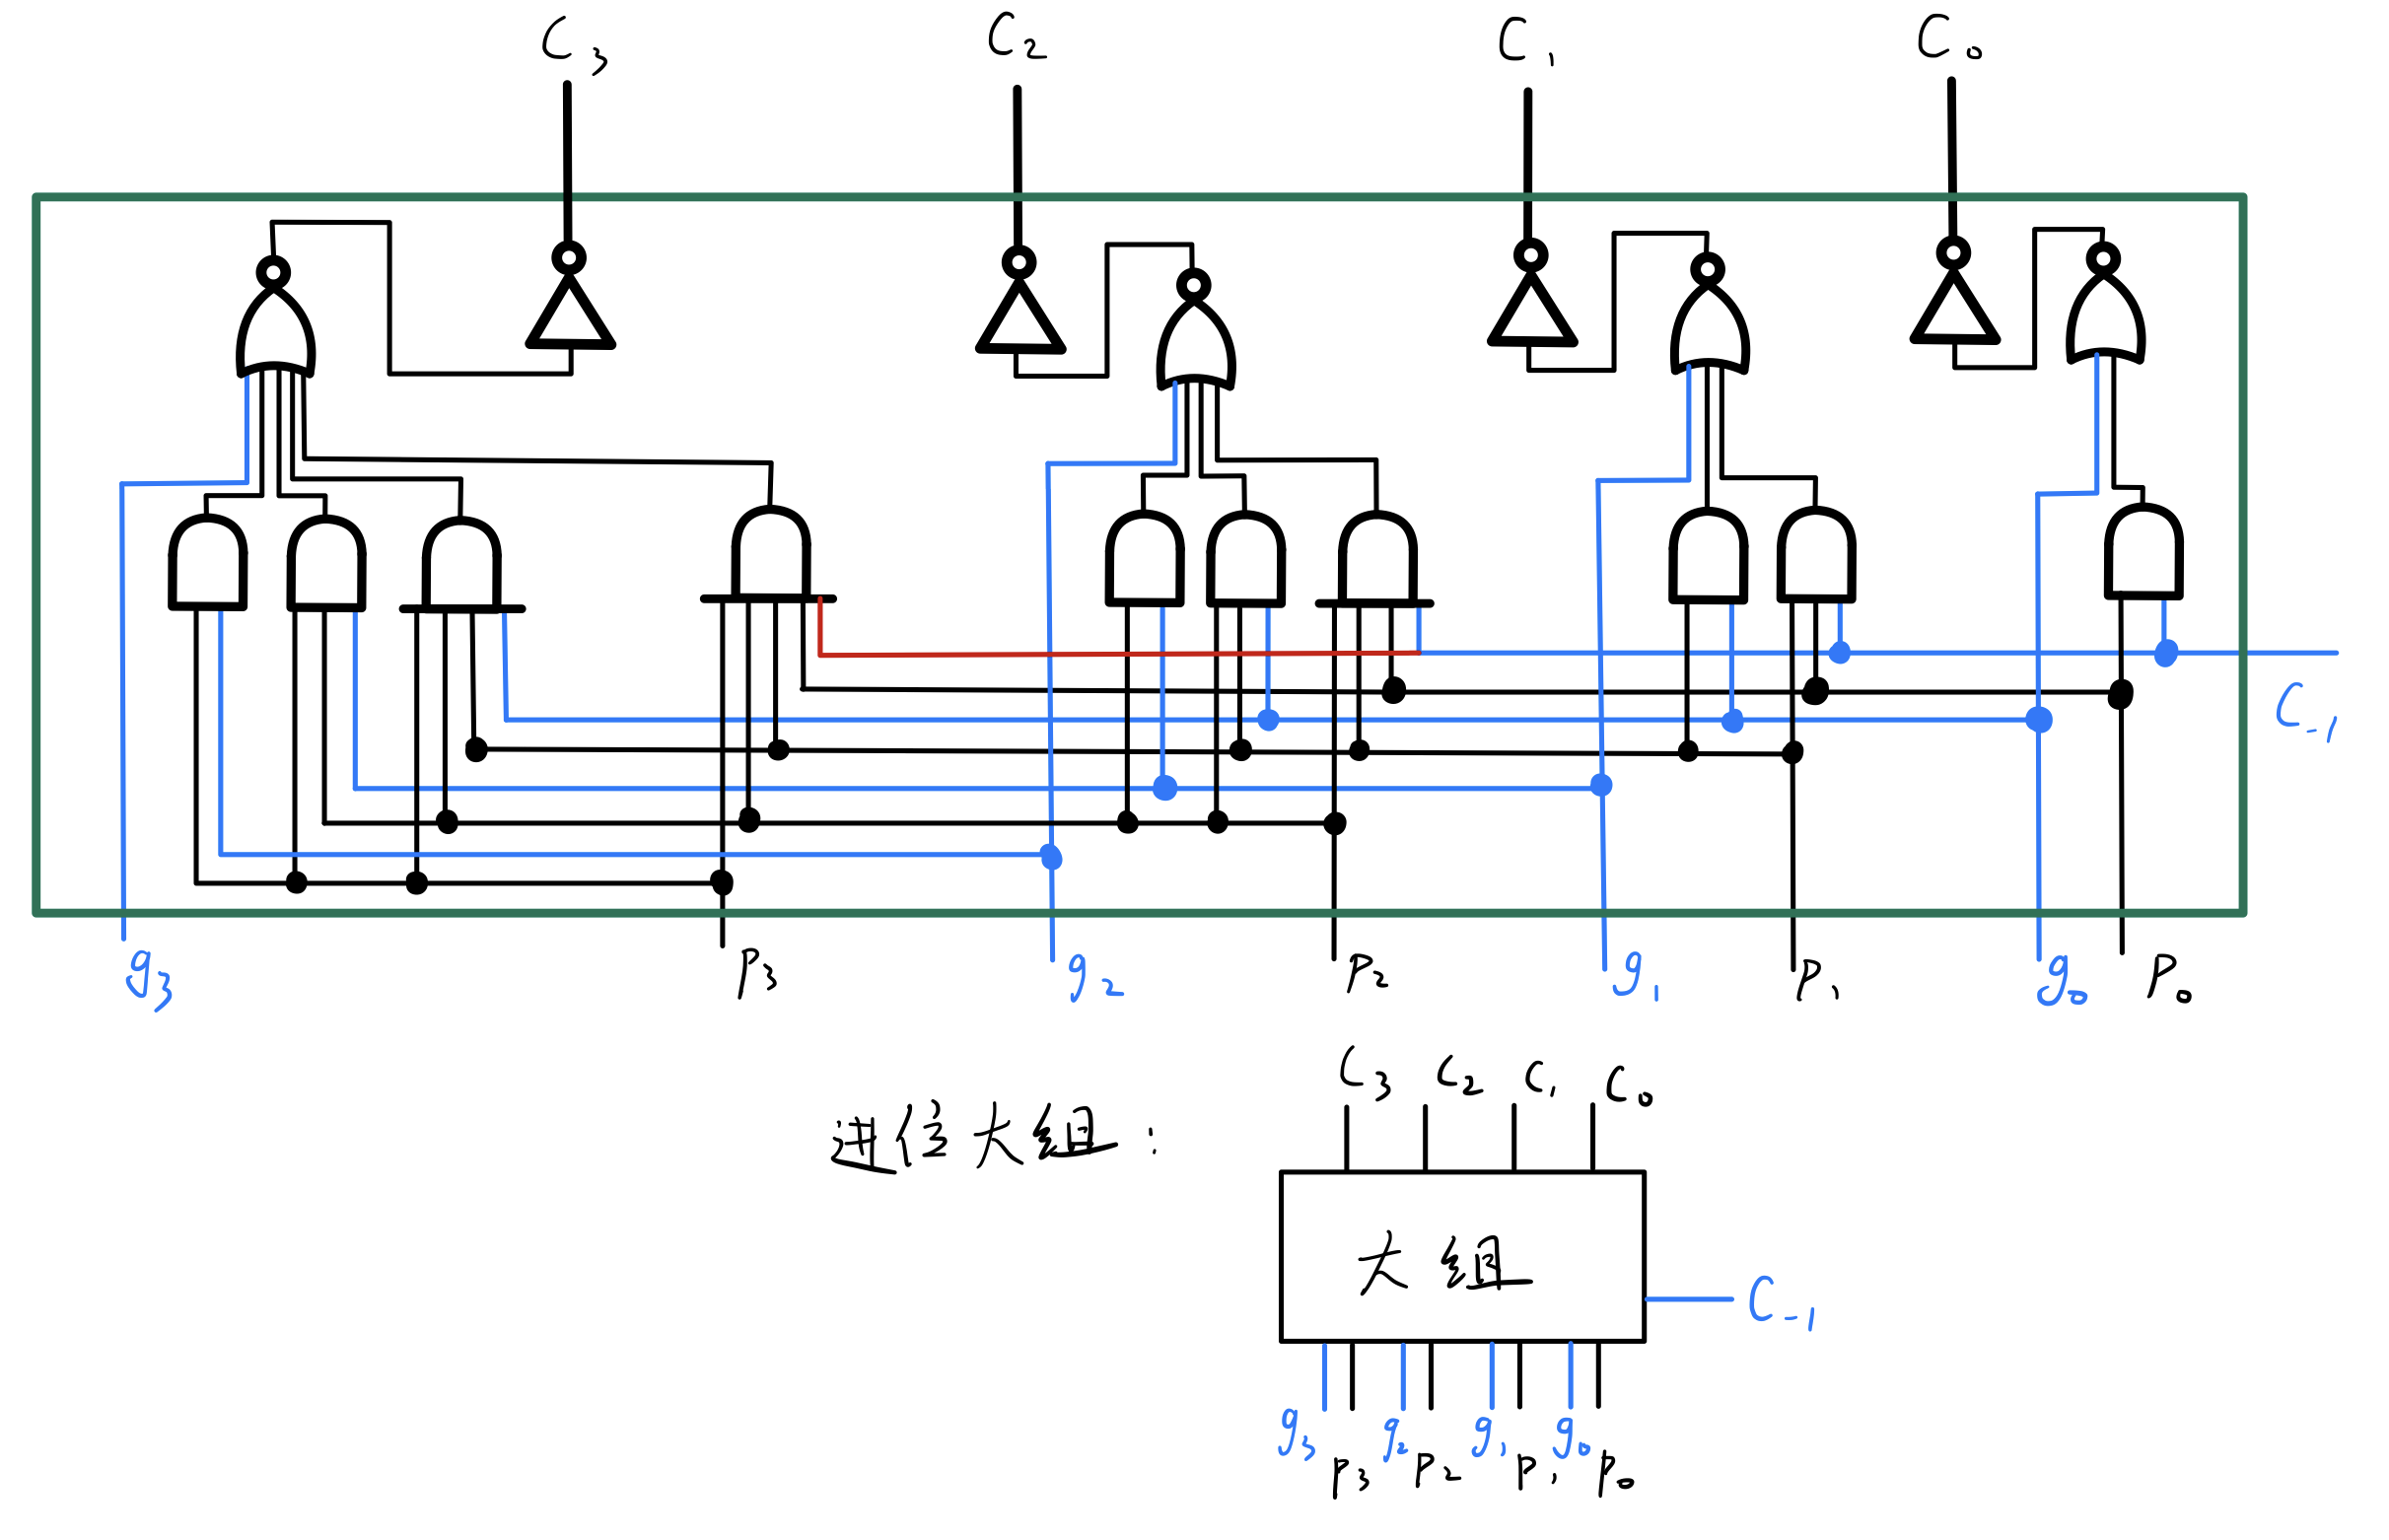
\includegraphics[width=10cm]{fig/6.31_大组.png}
        \caption{题6.31图1}
        \label{fig:6_31_1}
    \end{figure}
    \begin{figure}[!htbp]
        \centering
        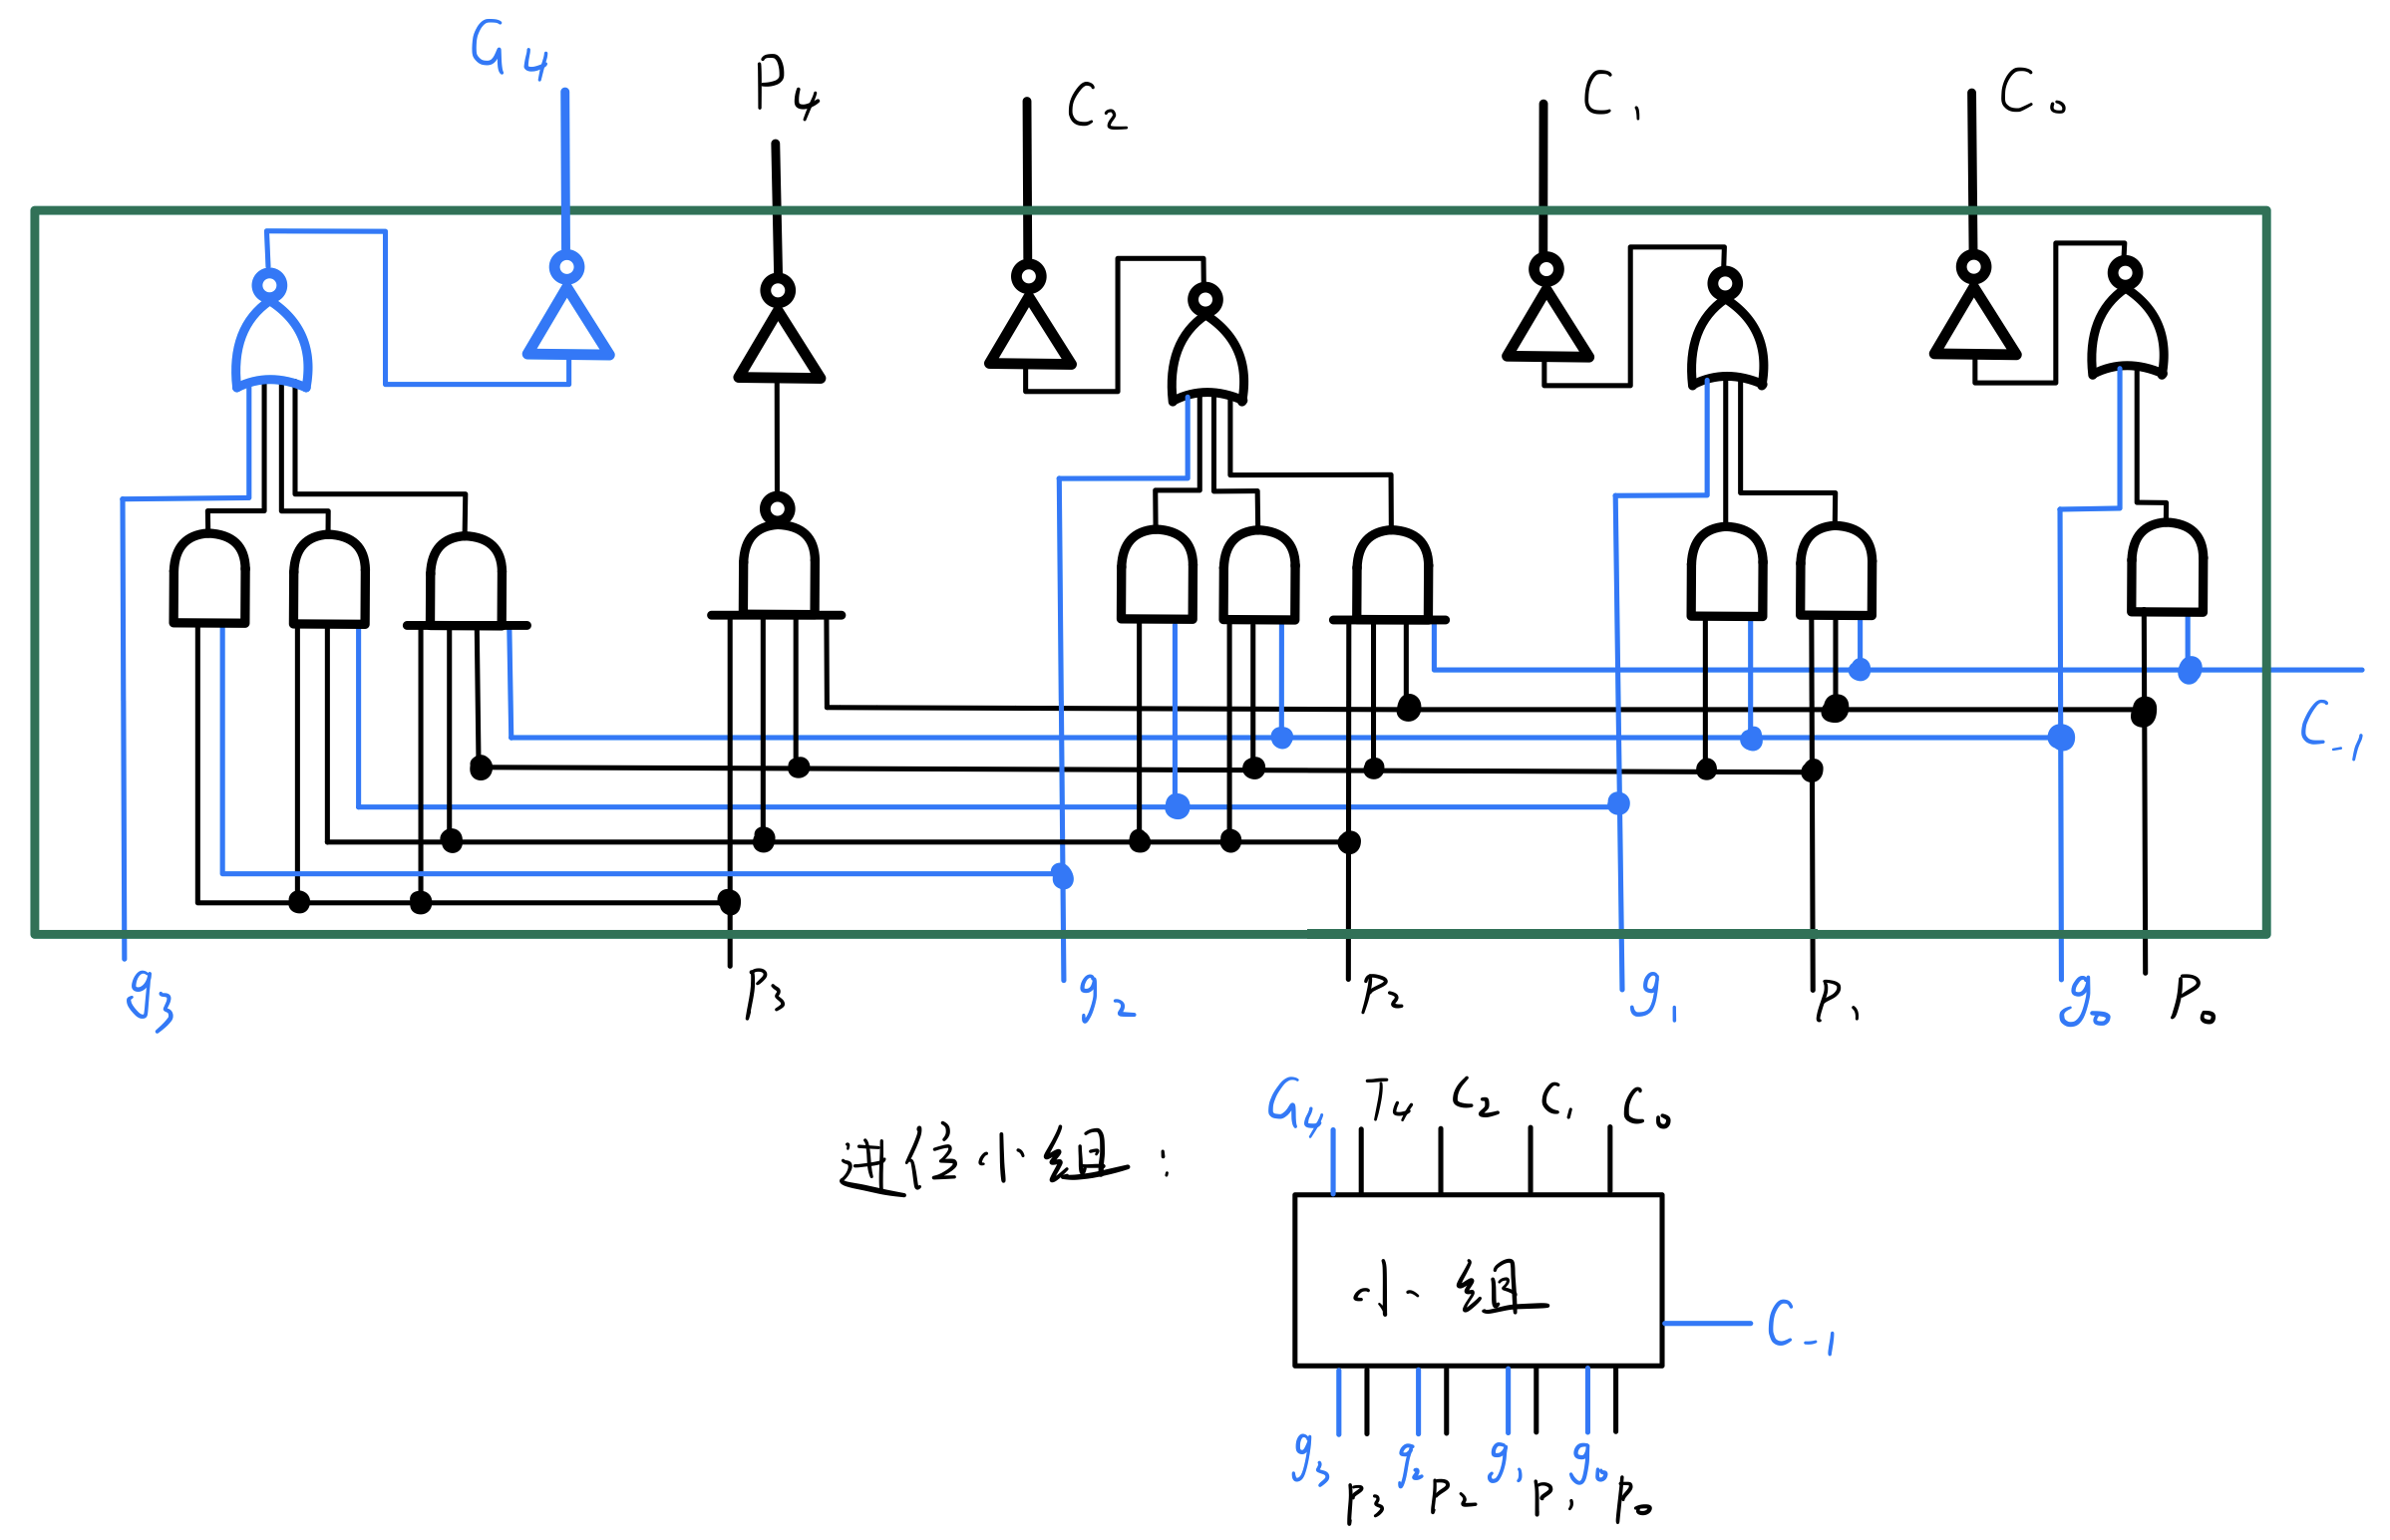
\includegraphics[width=10cm]{fig/6.31_小组.png}
        \caption{题6.31图2}
        \label{fig:6_31_2}
    \end{figure}
    \begin{figure}[!htbp]
        \centering
        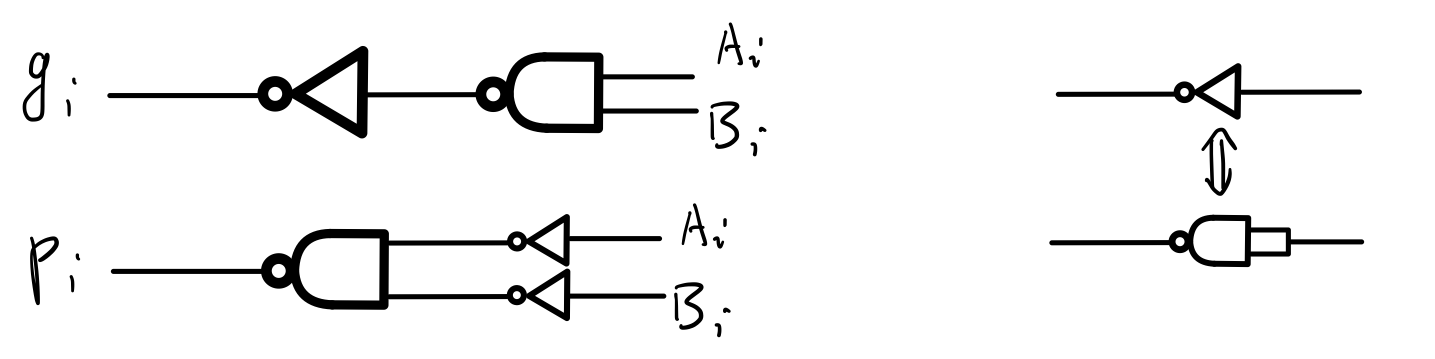
\includegraphics[width=5cm]{fig/6.31_表示.png}
        \caption{题6.31图3}
        \label{fig:6_31_3}
    \end{figure}
    \begin{figure}[!htbp]
        \centering
        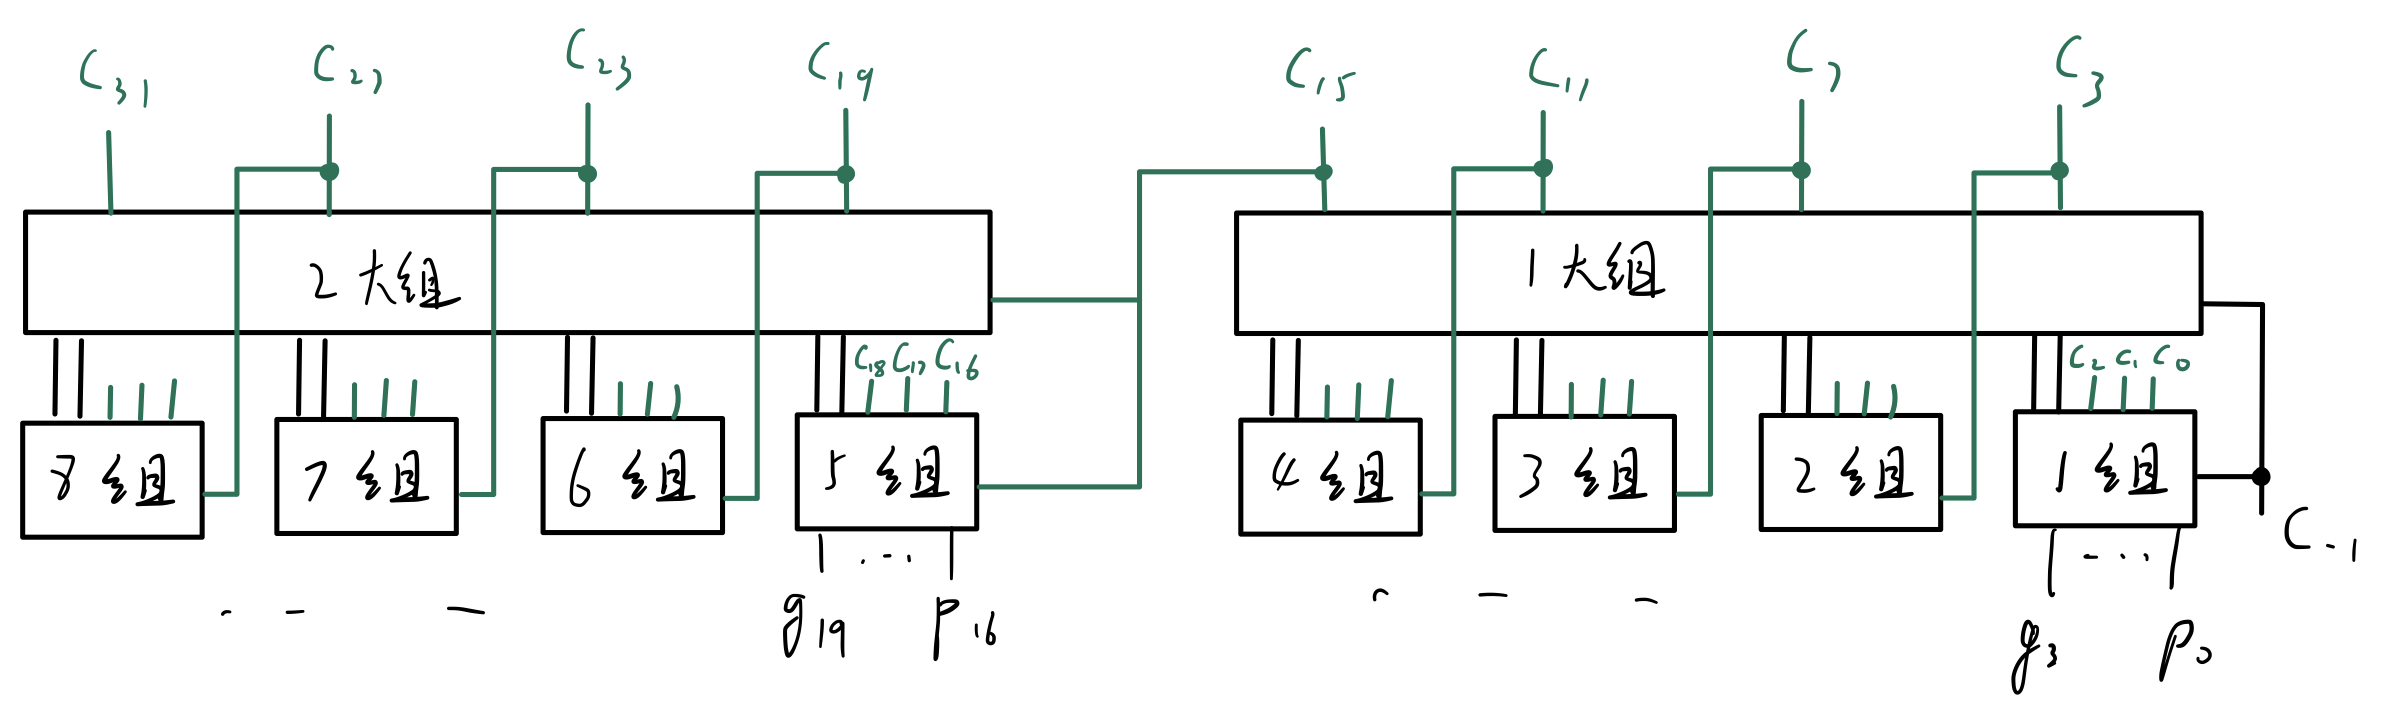
\includegraphics[width=10cm]{fig/6.31_进位链.png}
        \caption{题6.31图4}
        \label{fig:6_31_4}
    \end{figure}

    在图中, 所有非门都可以由与非门制成, 生成所有$g_i,\,p_i$需要$60 \unit{ns}$. 右侧的$D,T$、右侧大组的进位、左侧大组的进位、左侧小组的进位,各自需要$30+45=75 \unit{ns}$的时间. 一共需要$60 + 75*4 = 360 \unit{ns}$的时间来完成计算, 在限制时间之内.
\end{solution}
    













\end{document}